\chapter{Prologue}
This summer, we will be making our way through Knapp's \emph{Lie Groups
  Beyond an Introduction} \cite{knapp} although, I (the writer of these
notes) will occasionally refer to \cite{hall} for examples.

\section{Representation of Finite Groups}
\subsection{Definitions}
A \emph{representation} of a finite group $G$ on a finite-dimensional
complex vector space $V$ is a homomorphism $\rho\colon G\to\GL(V)$; we say
that such a map $\rho$ \emph{gives $V$ the structure of a $G$-module.} When
there is little ambiguity about the map $\rho$ we will call $V$ itself as a
representation of $G$; in this vein, we supress the symbol $\rho$ and write
$gv$ for $\rho(g)(v)$. The dimension of $V$ is sometimes called the
\emph{degree} of $\rho$.

A map $\varphi$ between two representations $V$ and $W$ of $G$ is a vector
space map $\varphi\colon V\to W$ such that
\begin{center}
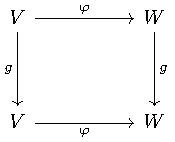
\includegraphics{figures/week-1-diag-1}
\end{center}
commutes for every $g\in G$. (We will call this a \emph{$G$-linear map}
when we want to distinguish it from an arbitrary linear map between the
vector spaces $V$ and $W$). We can then define $\Ker\varphi$,
$\Img\varphi$, and $\Coker\varphi$, which are also $G$-modules.

A \emph{subrepresentation} of a representation $V$ is a vector subspace $W$
of $V$ which is invariant under $G$. A representation $V$ is called
\emph{irreducible} if there is no proper nonzero invariant subspace $W$ of
$V$.

%%% Local Variables:
%%% mode: latex
%%% TeX-master: "../MA598-Lie-Groups"
%%% End:
